\documentclass{article}

% if you need to pass options to natbib, use, e.g.:
% \PassOptionsToPackage{numbers, compress}{natbib}
% before loading nips_2016
%
% to avoid loading the natbib package, add option nonatbib:
% \usepackage[nonatbib]{nips_2016}

\usepackage{nips_2016}
\usepackage{dsfont}

% to compile a camera-ready version, add the [final] option, e.g.:
% \usepackage[final]{nips_2016}

\usepackage[utf8]{inputenc} % allow utf-8 input
\usepackage[T1]{fontenc}    % use 8-bit T1 fonts
\usepackage{hyperref}       % hyperlinks
\usepackage{url}            % simple URL typesetting
\usepackage{booktabs}       % professional-quality tables
\usepackage{amsfonts}       % blackboard math symbols
\usepackage{nicefrac}       % compact symbols for 1/2, etc.
\usepackage{microtype}      % microtypography

\usepackage{listings}
\usepackage{amsthm}
% use Times
\usepackage{times}
% For figures
\usepackage{graphicx} % more modern
%\usepackage{epsfig} % less modern
\usepackage{subfig} 
\usepackage{fancyvrb}


\usepackage{caption}
\usepackage{subcaption}

\fvset{fontsize=\footnotesize}


\usepackage{multirow}
\usepackage{array}

\usepackage{amssymb}
\usepackage{listings}
\usepackage{wrapfig}
\usepackage{tabularx}


\usepackage{verbatim}
 \usepackage{booktabs}
 % For algorithms
\usepackage{algorithm}
\usepackage{algorithmic}
\usepackage{tikz}
% As of 2011, we use the hyperref package to produce hyperlinks in the
% resulting PDF.  If this breaks your system, please commend out the
% following usepackage line and replace \usepackage{icml2016} with
% \usepackage[nohyperref]{icml2016} above.
\usepackage{amsmath}
\usepackage{hyperref}
\DeclareMathOperator*{\argmin}{arg\,min} % thin space, limits underneath in displays
\DeclareMathOperator{\argmin}{argmin} % no space, limits underneath in displays



% Packages hyperref and algorithmic misbehave sometimes.  We can fix
% this with the following command.
\newcommand{\theHalgorithm}{\arabic{algorithm}}
\newcommand{\theSystem}{\textsc{ProgramSample}}

\newcommand{\Expect}{\mathds{E}} %{{\rm I\kern-.3em E}}
\newcommand{\Probability}{\mathds{P}} %{{\rm I\kern-.3em P}}

\newtheorem{proposition}{Proposition}

\newcommand\modt{\stackrel{\mathclap{\normalfont 2}}{\equiv}}


\title{Sampling for Bayesian Program Learning}

% The \author macro works with any number of authors. There are two
% commands used to separate the names and addresses of multiple
% authors: \And and \AND.
%
% Using \And between authors leaves it to LaTeX to determine where to
% break the lines. Using \AND forces a line break at that point. So,
% if LaTeX puts 3 of 4 authors names on the first line, and the last
% on the second line, try using \AND instead of \And before the third
% author name.

\author{
  David S.~Hippocampus\thanks{Use footnote for providing further
    information about author (webpage, alternative
    address)---\emph{not} for acknowledging funding agencies.} \\
  Department of Computer Science\\
  Cranberry-Lemon University\\
  Pittsburgh, PA 15213 \\
  \texttt{hippo@cs.cranberry-lemon.edu} \\
  %% examples of more authors
  %% \And
  %% Coauthor \\
  %% Affiliation \\
  %% Address \\
  %% \texttt{email} \\
  %% \AND
  %% Coauthor \\
  %% Affiliation \\
  %% Address \\
  %% \texttt{email} \\
  %% \And
  %% Coauthor \\
  %% Affiliation \\
  %% Address \\
  %% \texttt{email} \\
  %% \And
  %% Coauthor \\
  %% Affiliation \\
  %% Address \\
  %% \texttt{email} \\
}


\begin{SaveVerbatim}[]{ListSketch}
Program ::=
  (if Bool List
    (append RecursiveList
       RecursiveList RecursiveList))
Bool ::= (<= Int) | (>= Int)
Int ::= 0 | (1+ Int) | (1- Int)
      | (length List) | (head List)
List ::= a | nil | (filter Bool List)
      | (tail List) | (list Int)
RecursiveList ::= List | (recurse List)
\end{SaveVerbatim}

\begin{document}
% \nipsfinalcopy is no longer used

\maketitle

\begin{abstract}
  Towards learning programs from data, we introduce the problem of
  sampling programs from posterior distributions conditioned on that
  data. Within this setting, we propose an algorithm that uses a
  symbolic solver to efficiently sample programs.  The proposal
  combines constraint-based program synthesis with sampling via random
  parity constraints.  We give theoretical guarantees on how well the
  samples approximate the true posterior, and have empirical results
  showing the algorithm is efficient in practice, evaluating our
  approach on 22 program learning problems in the domains of text
  editing and computer-aided programming.
\end{abstract}

\section{Introduction}
\label{introduction}
Learning programs from examples is a central problem in artificial intelligence, and many recent approaches draw on techniques from machine learning.
Connectionist approaches, like the Neural Turing Machine~\cite{graves2014neural,DBLP:journals/corr/ReedF15,vinyals2015pointer} and symbolic approaches, like Hierarchical Bayesian Program Learning~\cite{lake2015human,DBLP:conf/icml/LiangJK10,menon2013machine},
couple a probabilistic learning framework with either gradient- or sampling-based search procedures.
In this work,
we consider the problem of Bayesian inference over program spaces.
We combine solver-based program synthesis~\cite{solar2008program} and sampling via random projections~\cite{ermon2013embed},
showing how to sample from posterior distributions over programs where the samples come from a distribution provably arbitrarily close to the true posterior. The new approach is implemented in a system called \theSystem{}
and evaluated on a set of program induction problems that include list 
and string manipulation routines. 


\subsection{Motivation and problem statement}
\newlength{\mylength}
\setlength{\mylength}{0.25cm}   % Saving fboxsep into mylength

\begin{wrapfigure}{r}{0.5\textwidth}
  \centering\vspace{-0.5cm}
\begin{tikzpicture}
\node[draw,rounded corners](problem)
     {\begin{tabular}{lr}
      Input & Output \\\hline
      ``1/21/2001'' & ``01''
     \end{tabular}};
\node[draw,rounded corners](sampledPrograms) at (0,-2)
     {\begin{tabular}{lr}
         {\ttfamily\small \hspace{-\mylength}substr(pos('0',-1),-1)} & ``last 0 til end'' \\
      {\ttfamily\small \hspace{-\mylength}const('01')}       & ``output 01''\\
      {\ttfamily\small \hspace{-\mylength}substr(-2,-1)} & ``take last two''
     \end{tabular}};
\draw[->,thick](problem.south) -- (sampledPrograms.north);
\end{tikzpicture}
  \caption{Learning string manipulation programs by example (top input/output pair). Our system receives data like that shown above and then sampled the different programs shown below (among others) from a description-length prior.}
  \label{ambiguous}
\end{wrapfigure}


Consider the problem of learning string edit programs, a well studied domain for programming by example.
Often end users provide these examples and are unwilling to give more than one instance,
which leaves the target program highly ambiguous.
One way of representing this ambiguity is to \emph{sample} string edit programs,
allowing us to learn from very few examples (Fig.~\ref{ambiguous})
and offer different plausible solutions.


  


Another program learning domain comes from \emph{computer-aided programming}, where the goal is to synthesize algorithms from
either examples or formal specifications.
This problem can be ill posed because many programs may satisfy the specification or examples.
When this ambiguity arises,
\theSystem{} proposes multiple implementations with a bias towards shorter or simpler ones.
The samples can also be used to efficiently approximate the posterior predictive distribution, effectively integrating out the program.
We show \theSystem{} learning counting routines and recursive sorting/reversing algorithms
while modeling the uncertainty over the correct algorithm.

Because any model can be represented as a (probabilistic or deterministic) program,
we need to carefully delimit
the scope of this work.
The programs we learn are a subset of those handled by constraint-based program synthesis tools.
This means that the program is \emph{finite} (bounded size, bounded runtime, bounded memory consumption),
can be modeled in a constraint solver (like a SAT or SMT solver),
and that the program's high-level structure is already given as a \emph{sketch}~\cite{solar2008program},
which can take the form of a recursive grammar over expressions.
The sketch defines the search space and imparts prior knowledge.
For example,
we use one sketch when learning string edit programs and a different sketch when learning recursive list manipulation programs.

More formally, our sketch specifies a finite set of programs, $S$,
as well as a measure of the programs' description length,
which we write as $\lvert x \rvert$ for $x\in S$.
%We assume description lengths are always natural numbers.
This defines a prior ($\propto 2^{- \lvert x \rvert }$).
For each program learning problem,
we have a specification (such as consistency with input/output examples)
and want to sample from $S$ conditioned upon the specification holding,
giving the posterior over programs $\propto 2^{- \lvert x \rvert } \mathds{1}[\text{specification holds for }x]$.
Throughout the rest of the paper, we write $p(\cdot )$ to mean this posterior distribution, and write $X$ to mean the set of all  programs in $S$  consistent with the specification.
So the problem is to sample from  $p(x) = \frac{2^{-|x|}}{Z}$  where $Z = \sum_{x\in X} 2^{-|x|}$.

We can invoke a \emph{solver}, which enumerates members of $X$,
possibly subject to extra constraints, but without any guarantees on
the order of enumeration.  Throughout this work we use a SAT solver,
and encode $x\in X$ in the values of $n$ Boolean decision variables.
With a slight abuse of notation we will use $x$ to refer to both a
member of $X$ and an assignment to those $n$ decision variables.  An
assignment to $j^{th}$ variable we write as $x_j$ for $1\leq j\leq n$.
Section~\ref{brisk} briskly summarizes this constraint-solving program synthesis technique.

\subsection{Program synthesis by constraint solving}\label{brisk}
The constraint solving approach to program synthesis, pioneered
in~\cite{solar2008program,srivastava2010program,jha2010oracle},
synthesizes programs by (1) modeling the space of programs as
assignments to Boolean decision variables in a constraint satisfaction
problem; (2) adding constraints to enforce consistency with a
specification; (3) asking the solver to find any solution to the
constraints; and (4) reinterpreting that solution as a program.

Fig.~\ref{booleanExample} illustrates this approach for for the toy
problem of synthesizing programs in a language consisting of
single-bit operators.  Each program has one input ($i$ in
Fig.~\ref{booleanExample}) which it transforms using \verb|nand|
gates. The recursive grammar in Fig.~\ref{booleanSketch} is the
sketch. If we inline the grammar, we can diagram the space of all
programs as an AND/OR graph (Fig.~\ref{booleanSpace}), where $x_j$ are
Boolean decision variables that control the program's structure.  For
each of the input/output examples (Fig.~\ref{booleanSpecification}) we
have constraints that model the program execution
(Fig.~\ref{booleanModel}) and enforce the desired output ($P_1$ taking
value $1$). After solving for a satisfying assignment to the
$x_j$'s, we can read these off as a program
(Fig.~\ref{booleanSolution}).  In this work we measure the description
length of a program $x$ as the number of bits required to specify its
structure (so $|x|$ is a natural number).\footnote{This is equivalent
  to the assumption that $x$ is drawn from a probabilistic grammar
  specified by the sketch}


\begin{SaveVerbatim}[]{ExampleSketch}
Program ::= i
| nand(Program,Program)
\end{SaveVerbatim}
\begin{SaveVerbatim}[]{ExampleSpecification}
Program(i = 0) = 1
\end{SaveVerbatim}

\begin{figure}
  \centering
\begin{tabular}{ccc}
  \subfloat[Sketch]{\fbox{{\BUseVerbatim[fontsize=\footnotesize,fontfamily=courier]{ExampleSketch}}}\label{booleanSketch}}&
  \multirow{-3}[2.5]{*}{\subfloat[Program space]{\fbox{\begin{tikzpicture}[level distance=1cm, grow=down,
    every node/.style={ thin},
    edge from parent/.style={-latex, thin, draw}
]
      \node (P) {$P_1$}
      child {node (Q) {$i$} edge from parent node[left] {$x_1\hphantom{i}$ }}
      child {node (S) {nand} 
    	child {node (e2) {$P_2$}
        	child {node {$i$} edge from parent node[left] {$x_2\hphantom{i}$}}
    		child {node (pp) {nand} edge from parent node[right] {$\hphantom{i}\overline{x}_2$}}
        }
        child {node (e3) {$P_3$}}
        edge from parent node[right] {$\hphantom{i}\overline{x}_1$}
    };
    \path (S) -- coordinate[midway] (PQ) (e2);
\path (S) -- coordinate[midway] (PR) (e3);
\draw (PQ) to[bend right=22] (PR);
\node (qq) [below] at (e3) {\vphantom{I}$\hdots\hdots$};
\node (ss) [below] at (pp) {\vphantom{I}$\hdots\hdots$};
  \end{tikzpicture}}\label{booleanSpace}}}&
  \subfloat[Specification]{\fbox{{\BUseVerbatim[fontsize=\footnotesize,fontfamily=courier]{ExampleSpecification}}}\label{booleanSpecification}}\\
  \subfloat[Constraints from program space]{\fbox{\[ \begin{aligned}
      &(c_1^1\vee c_2^1)\wedge \overline{(c_1^1\wedge c_1^2)}\\
      &      (c_2^1\vee c_2^1)\wedge\overline{(c_2^1\wedge c_2^2)}\\
&\cdots      \cdots
    \end{aligned} \]}\label{booleanExclusive}}
  &&
\subfloat[Constraints from specification]{\fbox{\[ \begin{aligned}
      &i\Leftrightarrow 0\wedge P_1\Leftrightarrow 1\\
      &x_1\Rightarrow (P_1\Leftrightarrow i)\\
      & \overline{x}_1\Rightarrow (P_1\Leftrightarrow \overline{P_2\wedge P_3})\\
      &\cdots\cdots
  \end{aligned} \]}\label{booleanModel}}\\
\multicolumn{3}{c}{\subfloat[Constraint solution; $|x| = 3$ bits]{\fbox{\[ \begin{aligned}
&x_1 = 0,\;x_2 = 1,\;x_3 = 1,\quad
\text{{\ttfamily Program = nand(i, i)}}
  \end{aligned} \]}\label{booleanSolution}}}
\end{tabular}
  \caption{Synthesizing a program via sketching and constraint solving. {\ttfamily Typewriter font} refers to pieces of programs or sketches, while math font refers to pieces of a constraint satisfaction problem.}
  \label{booleanExample}
\end{figure}


\subsection{Algorithmic contribution}
In the past decade different groups of researchers have  concurrently developed solver-based %\footnote{eg, Boolean satisfiability (SAT) solvers}
 techniques for (1) sampling of combinatorial spaces~\cite{gomes2006near,ermon2013embed,ermon2012uniform,chakraborty2014balancing} and (2) program synthesis~\cite{solar2008program,Gulwani:2011:SLP:1993498.1993506}.
This work unifies these two lines of research to attack the problem of program learning in a probabilistic setting.
We use program synthesis tools to convert a program learning problem into a SAT formula.
Then,
rather than search for one program (formula solution),
we augment the formula with random constraints that cause it to (approximately) sample the space of programs,
effectively ``upgrading'' our SAT solver from a program synthesizer to a program sampler.

While one could use a tool like Sketch to reduce a program learning problem to SAT
and then use an algorithm like PAWS, XORSample, or Unigen~\cite{ermon2013embed,gomes2006near,chakraborty2014balancing}
to sample programs from a description length prior,
doing so can be extremely inefficient\footnote{In many cases, slower than rejection sampling or enumerating all of the programs}.
Intuitively,
these solver-based samplers work by creating ``duplicate'' SAT solutions for high probability programs
such that uniform sampling of SAT solutions gives nonuniform sampling of programs.
When there are a few very likely (short) programs and many extremely unlikely (long) programs,
these techniques scale poorly. This poor scalability is because the ``duplication'' combines with the random constraints to entangle otherwise independent Boolean decision variables.
This phenomenon has been observed more generally when using these techniques to sample from large combinatorial spaces,
and is related to a quantity called the distribution's \emph{tilt}~\cite{chakraborty2014distribution}.
Previous work has relied on upper bounding the tilt.
Our main technical contribution is showing how to extend these techniques to distributions with high tilt,
such as those encountered in program synthesis problems.
%where there are often a few short, high-probability programs and many long, low-probability programs.

 


\section{The sampling algorithm}
Given the distribution $p(\cdot )$ on the program space $X$, it's
always possible to define a higher dimensional space $E$ (an
\emph{embedding}) and a mapping $F:E\to X$ such that sampling
uniformly from $E$ and applying $F$ will give us approximately
$p$-distributed samples~\cite{ermon2013embed}.
But, when the \emph{tilt} of $p(\cdot )$, defined
in~\cite{chakraborty2014distribution} as $\frac{\max_x p(x)}{\min_x p(x)}$,
becomes large, such an approach can be extremely
inefficient.\footnote{\cite{chakraborty2014distribution} take a qualitatively different approach from \cite{ermon2013embed} not based on an embedding, but which still becomes prohibitively expensive in the high-tilt regime.}

Our approach instead is to define an $F':E\to X$ such that uniform
samples on $E$ map to a distribution $q(\cdot )$ that is guaranteed to
have low tilt, but whose KL divergence from $p(\cdot )$ is low. The
discrepancy between the distributions $p(\cdot )$ and $q(\cdot )$ can
be corrected through rejection sampling. Sampling uniformly from $E$
is itself not trivial, but a variety of techniques exist to
approximate uniform sampling by adding random XOR constraints (random
projections mod 2) to the set $E$, which is extensively studied
in~\cite{gomes2006near,valiant1985np,chakraborty2014balancing,gomes2006model}.
These techniques introduce approximation error that can be made
arbitrarily small at the expense of lower
efficiency. Fig.~\ref{cartoon} illustrates this process.
\begin{wrapfigure}{R}{0.5\textwidth}\vspace{-0.5cm}\centering
  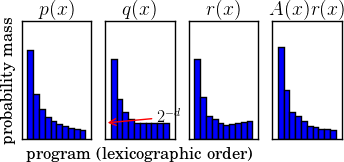
\includegraphics[width=0.5\textwidth]{cartoon_small.png}
  \caption{\theSystem{} twice distorts the posterior distribution $p(\cdot )$. First it introduces a parameter $d$ that bounds the tilt; we correct for this by accepting samples w.p. $A(x)$. Second it samples from $q(\cdot )$ by drawing instead from $r(\cdot )$, where $KL(q||r)$ can be made arbitrarily small by appropriately setting another parameter, $K$. The distribution of samples is $A(x)r(x)$.}\label{cartoon}\vspace{-0.5cm}
\end{wrapfigure}

\subsection{Getting high-quality samples}
\textbf{Low-tilt approximation.}
We introduce a parameter into the sampling algorithm, $d$, that parameterizes $q(\cdot )$.
The parameter $d$ acts as a threshold, or cut-off, for the description length of a program;
the distribution $q(\cdot )$ acts as though any program with description length exceeding $d$ can be encoded using $d$ bits. Concretely,
\begin{equation}
  q(x) \propto \begin{cases}
    2^{-\lvert x \rvert },& \text{if } \lvert x \rvert \leq d\\
    2^{-d},              & \text{otherwise}
\end{cases}
  \end{equation}
If we could sample exactly from $q(\cdot )$, we could reject a sample $x$ with probability $1-A(x)$ where $A$ is
\begin{equation}
  A(x) \propto \begin{cases}
    1,& \text{if } \lvert x \rvert \leq d\\
    2^{-\lvert x \rvert +d},              & \text{otherwise}
    \end{cases}
  \end{equation}
and get exact samples from $p(\cdot )$, where the acceptance rate would approach 1 exponentially quickly in $d$. We have the following:
\begin{proposition}\label{acceptanceBound}
  Let $x\in X$ be a sample from $q(\cdot )$. The probability of accepting $x$ is at least $\frac{1}{1 + |X|2^{\lvert x_* \rvert -d}}$ where $x_* = \argmin_x \lvert x \rvert $.
\end{proposition}

%Two comments on Prop.~\ref{acceptanceBound}: (1) $Z$ is difficult to compute, and so we will use loose lower bounds; in fact $Z > 2^{-\lvert x_* \rvert }$ is sufficient for our later needs.
%A similar argument also shows that the KL between $p(\cdot )$ and $q(\cdot )$ is order $2^{-d}\frac{|X|}{Z}$.

The distribution $q(\cdot )$ is useful because we can guarantee that it has tilt bounded by
$2^{d - \lvert x_* \rvert }$.
%Recent work has shown that the performance of nonuniform sampling via random projections degrades as the tilt increases~\cite{chakraborty2014distribution};
Introducing the proposal $q(\cdot )$ effectively reifies the tilt,
making it a parameter of the sampling algorithm,
not the distribution over programs.
We now show how to approximately sample from $q(\cdot )$ using a variant of the Embed and Project framework~\cite{ermon2013embed}.

\textbf{The embedding.} The idea is to define a new set of programs, which we call $E$, such that short programs are included in the set much more often than long programs.
Each program $x$ will be represented in $E$ by an amount proportional to $2^{-\min (\lvert x \rvert ,d)}$, thus proportional to $q(x)$,
such that sampling elements uniformly from $E$  samples according to $q(\cdot )$.

We embed $X$ within the larger set $E$ by introducing $d$ \emph{auxiliary variables}, written $(y_1,\cdots, y_d)$,
such that every element of $E$ is a tuple of an element of $x = (x_1,\cdots , x_n )$ and an assignment to $y = (y_1,\cdots, y_d)$:
  \begin{equation}
    E = \{(x,y) \text{ }:\text{ } x\in X,  \bigwedge_{1\leq j \leq d} \lvert x \rvert \geq j\Rightarrow y_j=1 \}
  \end{equation}
  Suppose we sample $(x,y)$ uniformly from $E$.
  Then the probability of getting a particular $x\in X$ is proportional to
  $|\{(x',y)\in E \text{ : } x' = x\}| = |\{y\text{ : } \lvert x \rvert \geq j\Rightarrow y_j=1\}|=2^{\min (0,d-\lvert x \rvert )}$ 
  which is proportional to $q(x)$. Notice that $|E|$ grows exponentially with $d$, and thus with the tilt of the $q(\cdot )$. This is the crux of the inefficiency of sampling from high-tilt distributions in these frameworks:
  empirically, generating uniform samples using random projections, described below, becomes inefficient when the size of the support of the distribution is very high.

  \textbf{The random projections.} We  could sample exactly from $E$  by invoking the solver $|E|+1$ times to get every element of $E$,
  but in general it will have $O(|X|2^d)$ elements, which could be very large.
  Instead, we ask the solver for all the elements of $E$ consistent with $K$ random constraints
  such that (1) few elements of $E$ are likely to satisfy (``survive'') the constraints,
  and (2) any element of $E$ is approximately equally likely to satisfy the constraints.
  We can then sample a survivor uniformly to get an approximate sample from $E$, an idea introduced in the XORSample$'$ algorithm~\cite{gomes2006near}.
  Although simple compared to recent approaches~\cite{chakraborty2014balancing,ermon2014low,achlioptas2015stochastic}, it suffices for our theoretical and empirical results.

  Our random constraints take the form of XOR, or parity constraints, which are random projections mod 2.
  Each constraint fixes the parity of a random subset of SAT variables in $x$ to either 1 or 0;
  thus any $x$ survives a constraint with probability $\frac{1}{2}$.
  A useful feature of random parity constraints is that whether an assignment to the SAT variables survives is independent of whether another, different assignment survives, which has been exploited to create a variety of approximate sampling algorithms~\cite{gomes2006near,valiant1985np,chakraborty2014balancing,gomes2006model}.
  
  Then the $K$ constraints are of the form $h\left(\begin{smallmatrix}x\\y\end{smallmatrix}\right) \modt b$ where $h$ is a $K\times (d+n)$ binary matrix and $b$ is a $K$-dimensional binary vector.
  If no solutions satisfy the $K$ constraints then the sampling attempt is rejected.
  These samples are close to uniform in the following sense, which strengthens previous analyses: %, which strengthens the result in~\cite{gomes2006near}.
  \begin{proposition}\label{propositionLowerBound}
    The probability of sampling $(x,y)$ is at least $\frac{1}{|E|}\times \frac{1}{1 + 2^K/|E|}$ and the probability of getting any sample at all is at least $1 - 2^{K}/|E|$.
  \end{proposition}

  So we get approximate samples from $E$ as long as $|E|2^{-K}$ is not small.
  In reference to Fig.~\ref{cartoon},
  we call the distribution of these samples $r(x)=\sum_y r(x,y)$.
  Schemes more sophisticated than XORSample$'$, like~\cite{ermon2013embed}, also guarantee upper bounds on sampling probability, but we found that these were unnecessary for our main result, which is that the KL between $p(\cdot )$ and $A(x)r(x)$ goes to zero exponentially quickly in a new quantity we call $\Delta$:
  \begin{proposition}\label{mainResult}
    Write $Ar(x)$ to mean the distribution  proportional to $A(x)r(x)$. Then $D(p||Ar)<\log \left( 1 + \frac{1 + 2^{ - \gamma}}{1 + 2^\Delta}\right)$ where
    $\Delta = \log |E| - K$ and $\gamma = d - \log |X| - \lvert x_* \rvert $.
  \end{proposition}

  So we can approximate the true distribution $p(\cdot )$ arbitrarily well, but at the expense of either a larger embedding or more calls to the solver.
  The supplement contains more thorough theoretical and empirical analyses of this accuracy/runtime trade-off.
%  Here we depart from the Unigen and Uniwit families of approaches~\cite{chakraborty2014distribution,chakraborty2014balancing} which only guarantee that the distribution of samples is with in a factor of 6.84 of the target distribution.
%  Other approaches, like PAWS~\cite{ermon2013embed}, can prove analogously strong bounds.

  Proposition~\ref{mainResult} requires knowing $\min_x \lvert x \rvert $ to set $K$ and $d$. We compute $\min_x \lvert x \rvert $ using the iterative minimization routine in~\cite{singh2013automated}; in practice this is very efficient for finite program spaces. We also need to calculate $|X|$ and $|E|$, which are model counts that are in general difficult to compute exactly.
  However, many approximate model counting schemes exist, which provide upper and lower bounds that hold with arbitrarily high probability.
  We use Hybrid-MBound~\cite{gomes2006model} to upper bound $|X|$ and lower bound $|E|$ that each individually hold with probability at least $1-\delta / 2$ (see Alg.~\ref{mainAlgorithm}), thus
  giving lower bounds on both the $\gamma$ and $\Delta$ parameters of Proposition~\ref{mainResult} with probability at least $1-\delta$
  and thus an upper bound on the KL divergence. 

   
  \begin{algorithm}[tb]
   \caption{\theSystem{}}
   \label{mainAlgorithm}
\begin{algorithmic}
  \STATE {\bfseries Input:} Program space $X$, number of samples $N$, failure probability $\delta$, parameters $\Delta > 0$, $\gamma > 0$
  \STATE {\bfseries Output:} $N$ samples 
  \STATE Set $\lvert x_* \rvert  = \min_{x\in X} \lvert x \rvert $
  \STATE Set $B_X = $ ApproximateUpperBoundModelCount($X$,$\delta/2$)
  \STATE Set $d = \lceil \gamma + \log B_X + |x_* |\rceil$
  \STATE Define $E = \{(x,y) \text{ }:\text{ } x\in X,  \bigwedge_{1\leq j \leq d}  \lvert x \rvert \geq j\implies A_j=1 \}$
  \STATE Set $B_E = $ ApproximateLowerBoundModelCount($E$,$\delta/2$)
  \STATE Set $K = \lfloor \log B_E - \Delta \rfloor $
  \STATE Initialize samples $ = [\hspace{0.05cm}]$
  \REPEAT
  \STATE Sample $h$ uniformly from $\{0,1\}^{(d+n)\times K}$
  \STATE Sample $b$ uniformly from $\{0,1\}^{K}$
  \STATE Enumerate $\mathcal{S} = \{ (x,y) \text{ where } h(x,y) = b \wedge x\in X\}$
  \IF{$|\mathcal{S}| > 0$}
  \STATE Sample $(x,y)$ uniformly from $\mathcal{S}$
  \IF{Uniform$(0,1) < 2^{d - \lvert x \rvert }$}
  \STATE samples $ = \text{samples}+ [x]$
  \ENDIF
   \ENDIF
   \UNTIL{$|\text{samples}| = N$}
   \STATE {\bfseries return} samples
\end{algorithmic}
  \end{algorithm}



 

     
  \section{Experimental results}

  We evaluated \theSystem{} on program learning problems in a text editing domain and a list manipulation domain.
  For each domain, we wrote down a sketch and produced SAT formulas using the tool in~\cite{solar2006combinatorial}, specifying a large but finite set of possible programs.
  This implicitly defined a description-length prior, where $\lvert x \rvert $ is the number of bits required to specify $x$ in the SAT encoding.
We used   CryptoMiniSAT~\cite{crypto}, which can efficiently handle parity constraints.
  

\subsection{Learning Text Edit Scripts}
We applied our program sampling algorithm to a suite of programming by
demonstration problems within a text editing domain.  Here, the
challenge is to learn a small text editing program from very few
examples and apply that program to held out inputs.  This problem is
timely, given the widespread use of the Flashfill program synthesis
tool, which now ships by default in Microsoft Excel~\cite{real_world}
and can learn sophisticated edit operations in real time from
examples.  We modeled a subset of the
Flashfill~\cite{Gulwani:2011:ASP:1926385.1926423} language; our goal
here is not to compete with Flashfill, which is heavily engineered for
its specific domain, but to study the behavior of our more
general-purpose program learner in a real-world task.  To impart
domain knowledge, we used a sketch equivalent to the grammar in Fig.~\ref{textGrammar}.

\begin{SaveVerbatim}[]{TextSketch}
Program ::= Term | Program + Term
Term    ::= String | substr(Pos,Pos)
Pos     ::= Number
         |  pos(String,String,Number)
Number  ::= 0 | 1 | 2 | ... 
         | -1 | -2 | ...
String  ::= Character 
         |  Character + String
Character ::= a | b | c | ...
\end{SaveVerbatim}

\begin{wrapfigure}{R}{0.5\textwidth}\centering
  \BUseVerbatim[fontsize=\footnotesize,fontfamily=courier]{TextSketch}
  \caption{The sketch (program space) for learning text edit scripts}\label{textGrammar}
\end{wrapfigure}

Because FlashFill's training set is not yet public, we drew text editing problems from~\cite{DBLP:conf/ecai/LinDETM14} and adapted them to our subset of FlashFill, giving 19 problems, each with 5 training examples.
The supplement contains these text edit problems.

We are interested both in the ability of the learner to generalize
and in \theSystem{}'s ability to generate samples quickly.
Tbl.~\ref{listTimes} shows the average time per sampling attempt using \theSystem{}, which is on the order of a minute.
These text edit problems come from distributions with extremely high tilt: often the smallest program is only tens of  bits long, but the program space contains (implausible) solutions with over 100 bits.
 By putting $d$ to $\lvert x_* \rvert -n$ we eliminate the tilt correction and recover a variant of the approaches in~\cite{ermon2013embed}. % (todo: is 2014 actually a variant of this?). chakraborty2014distribution
This baseline does not produce any samples for any of our text edit problems in under an hour.\footnote{Approximate model counting of $E$ was also intractable in this regime, so we used the lower bound $|E|\geq 2^{d-\lvert x_* \rvert } + |X| - 1$}

The learner generalizes to unseen examples, as Fig.~\ref{flashPerformance} shows.
We evaluated the performance of the learner on held out test examples while varying training set size, and compare with baselines that either (1) enumerate programs in the arbitrary order provided by the underlying solver,
or (2) takes the most likely program under $p(x)$ (MDL learner).
The posterior is sharply peaked,
with most samples being from the MAP solution,
and so our learner does about as well as the MDL learner.
However,
sampling offers an (approximate) predictive posterior over solutions to the held out examples;
in a real world scenario, one would offer the top $C$ solutions to the user
and let them choose,
much like how spelling correction works.
This procedure allows us to offer the correct solutions more often than the MDL learner (Fig.~\ref{mdl}), because we correctly handle ambiguous problems like in Fig.~\ref{ambiguous}.
\begin{figure}\centering
  \begin{minipage}{0.45\textwidth}
    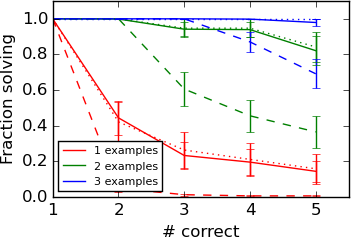
\includegraphics[width=0.7\textwidth]{smallFractionSolving.png}
  \caption{Generalization when learning text edit operations by example. Results averaged across 19 problems. Solid: 100 samples from \theSystem{} . Dashed: enumerating 100 programs. Dotted: MDL learner. Test cases past 1 (resp. 2,3) examples are held out when trained on 1 (resp. 2,3) examples.}\label{flashPerformance}        \end{minipage}%
\hspace{0.1\textwidth}\begin{minipage}{0.45\textwidth}\centering
    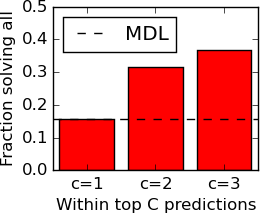
\includegraphics[width=0.6\textwidth]{small_mdl.png}
    \caption{Comparing the MDL learner (dashed black line) to program sampling when doing one-shot learning. We count a problem as ``solved'' if  the correct joint prediction to the test cases is in the top $C$ most frequent samples.}\label{mdl}
  \end{minipage}
 \end{figure}
\pagebreak
\begin{figure}\centering
  \begin{minipage}{0.5\textwidth}
    \centering
    \captionof{table}{Average solver time to generate a sample measured in seconds. See Fig.~\ref{listCurves} and \ref{flashPerformance} for training set sizes.}
    \label{listTimes}
    \begin{tabular}{llll}
      &      Large set      &  Medium set          &     Small set\\\hline
      text edit&49\pm 3 &21 \pm 1 &84 \pm 3 \\
      sort    & 1549\pm 155 & 905 \pm 58   & 463 \pm 65  \\
      reverse & 326\pm 42    & 141 \pm 18  &      39 \pm 3      \\
      count        &    $\leq 1$          &   $\leq 1$          &          $\leq 1$
    \end{tabular}
  \end{minipage}%
  \hspace{0.9cm}\begin{minipage}{0.4\textwidth}
  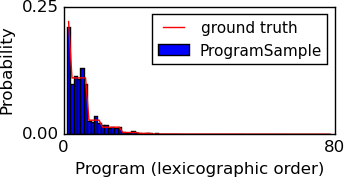
\includegraphics[width=\textwidth]{small_probabilityPlot.png}
  \caption{Sampling frequency vs. ground truth probability for 1000 runs of \theSystem{} on a counting task.}
  \label{marginal}
    \end{minipage}
\end{figure}



\subsection{Learning list manipulation algorithms}

One goal of program synthesis is \emph{computer-aided programming}~\cite{solar2008program}, where a program induction system automatically generates executable code from either declarative specifications or examples of desired behavior.
Systems with this goal has been successfully applied to, for example, synthesizing intricate bitvector routines from specifications~\cite{gulwani2011automating}.
However, when learning from examples, there is often uncertainty over the correct program.
While past approaches have handled this uncertainty within an optimization framework (see~\cite{raychev2016learning,ellis2015unsupervised,singh2013automated}),
we show that \theSystem{} can \emph{sample} algorithms.
\begin{wrapfigure}{r}{0.5\textwidth}\centering
  \begin{minipage}{0.5\textwidth}
    \BUseVerbatim[fontsize=\footnotesize,fontfamily=courier]{ListSketch}
  \captionof{figure}{The sketch (program space) for learning list manipulation routines}\label{ListGrammar}
  \end{minipage}
  
\vspace{\baselineskip}
\vspace{\baselineskip}

\begin{minipage}{0.5\textwidth}
    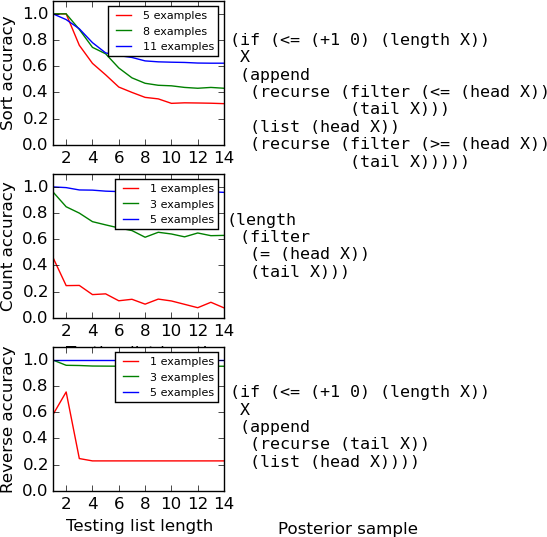
\includegraphics[width=\textwidth]{tinyList.png}
  \caption{Generalization of the  learner on list manipulation tasks. Trained on random lists of length $\leq 3$.}
  \label{listCurves}
\end{minipage}
\end{wrapfigure}
We take as our goal to learn recursive routines for sorting, reversing, and counting list elements from input/output examples,
particularly in the ambiguous,
unconstrained regime of few examples.
We used a sketch  with a set of basis primitives capable of representing a range of list manipulation routines equivalent to the grammar in Fig.~\ref{ListGrammar}.






A description-length prior that penalizes longer programs allowed learning of recursive list manipulation routines (from production \verb|Program|) and a non-recursive count routine (from production \verb|Int|); see Fig.~\ref{listCurves},
which shows average accuracy on held out test data when trained on variable numbers of short randomly generated lists.
With the large training set (5--11 examples) \theSystem{} recovers a correct implementation,
and with less data it recovers a distribution over programs
that functions as a probabilistic algorithm despite being composed of only deterministic programs.


For some of these program learning tasks the number of consistent programs is small enough that we can enumerate all of them, allowing us to compare our sampler with the ground-truth probabilities.
Fig.~\ref{marginal} shows this comparison for a counting problem with 80 consistent programs, showing empirically that the tilt correction and random constraints do not significantly perturb the distribution.

Tbl.~\ref{listTimes} shows the average solver time per sample; we see that generating recursive routines like sorting and reversing is much more costly than generating the nonrecursive counting routine.
The constraint-based approach propositionalizes higher-order constructs like recursion, and so reasoning about them is much more costly.



\pagebreak
\section{Discussion}

\subsection{Related work}
There is a vast literature on program learning within the AI and machine learning communities.
Many employ a (possibly stochastic) heuristic search over structures using genetic programming~\cite{DBLP:books/daglib/0070933} or MCMC~\cite{schkufza2013stochastic}.
These approaches often find good programs and can discover more high-level structure than our approach.
However, they are prone to getting trapped in local minima
and, when used as a sampler, determining the mixing time is in general not possible.
Recently researchers have turned to the problem of learning good priors over programs in a multitask setting~\cite{DBLP:conf/icml/LiangJK10,menon2013machine,Dechter:2013:BLV:2540128.2540316}.
We see our work here as particularly complementary to these methods: while they focus on learning the structure of the hypothesis space,
we focus on efficiently sampling an already given hypothesis space (the sketch).
There are several recent proposals for recurrent deep networks that learn algorithms~\cite{DBLP:journals/corr/ReedF15,graves2014neural}.
We see our system working in a different regime,
where we want to quickly learn an algorithm from a small number of examples or an ambiguous specification.

The program synthesis community has several recently proposed learners that work in an optimization framework~\cite{raychev2016learning,ellis2015unsupervised,singh2013automated}.%, and these motivate our description length prior.
By computing a posterior over programs, we can more effectively represent uncertainty, particularly in the small data limit, but at the cost of more computation.%: our algorithm requires an optimization routine to calibrate the sampler.


\theSystem{} borrows heavily from a line of work started
in~\cite{gomes2006near,gomes2006model} on sampling of combinatorial
spaces using random XOR constraints, which is motivated by results in
complexity theory~\cite{valiant1985np}.  An exciting, recent approach
is to use \emph{sparse} XOR constraints for discrete integration and
sampling~\cite{ermon2014low,achlioptas2015stochastic}, which might  sample more efficiently from our embedding of the program
space.

\subsection{Limitations of the approach}

The constraint-based synthesis methods on which our technique is built tend to excel in domains where the structure of the expected solutions can be restricted by a sketch~\cite{solar2008program} and where much of the program's description length can be easily computed from the program text. 
For example, \theSystem{} can synthesize text editing programs taking almost 60 bits of description length in a couple seconds, but spends 10 minutes synthesizing a recursive sorting routine that takes fewer bits of description length but where the program structure is less restricted. 
Constraint-based methods also require the entire problem to be represented symbolically, so they have trouble when the function to be synthesized involves complex building blocks such as numerical routines that are difficult to analyze.
For such problems, methods based on stochastic search~\cite{nori2015efficient,schkufza2013stochastic,DBLP:books/daglib/0070933} can be more effective because they only need to be able to run the functions under consideration. Finally, past work has also shown empirically that constraint-based approaches scale poorly with data set size, although this can be mitigated with clever approaches that consider data incrementally ~\cite{ellis2015unsupervised,raychev2016learning}.


The requirement of producing representative samples imposes some
additional overheads on our approach, so scalability can more limited
than for standard symbolic techniques on some problems. For example,
our method requires 1 MAP inference query, and 2 queries to an
approximate model counter for every new problem. The approximate model
counter serves to ``calibrate'' the sampler, and its cost can be
amortized because it only has to be invoked twice in order to generate
an arbitrary number of iid samples. Approximate model counters like
ApproxMC~\cite{approximatemc} have complexity comparable with that of
generating a sample, but the complexity is strongly dependent on the
number of solutions to the system.  Thus, for good performance,
\theSystem{} requires that there not be too many programs consistent
with the data---the largest spaces considered in our experiments had
$\leq 10^7$ programs. This limitation, together with the general
performance characteristics of symbolic techniques, means that the
approach will work best for ``needle in a haystack'' problems, where
the space of possible programs is large but restricted in its
structure, and where only a small fraction of those programs satisfy
the semantics constraints.


\subsection{Future work}
This work could naturally extend to other domains that involve inducing latent symbolic structure from small amounts of data,
such as semantic parsing to logical forms~\cite{liang11dcs},
synthesizing motor programs~\cite{lake2015human},
or learning relational theories~\cite{logical}.
These applications have some component of transfer learning,
and building efficient program learners that can transfer inductive biases across tasks is a prime target for future research.

\bibliographystyle{unsrt}
{\small \bibliography{main}}

\end{document}
